% @author Marcel Ruland (2018)
% !TEX encoding = UTF-8 Unicode
% !TEX TS-program = LuaLaTeX
\documentclass[aspectratio=169]{beamer}
%\setbeameroption{show notes}


%*******************Beamer Theme*******************
\usetheme{Dresden}				% use Dresden theme
\useinnertheme{rectangles}		% rectangles for itemize environment etc
\useoutertheme{infolines}		% lots of info using little space
\setbeamercovered{transparent}	% set covered items to 85% alpha
%**************************************************

%******************Packages in Use*****************
\usepackage[english]{babel}						% English language support
\usepackage{ttjenevers}							% use TT Jenevers for rm
\usepackage{ttcommons}							% use TT Commons for sf
\setmonofont[Scale=MatchLowercase]{Envy Code R}	% use Envy Code R for tt
\usepackage{microtype}							% improved typography
\usepackage{natbib}								% bibliography
\bibliographystyle{newharvard}					% custom Harvard bibliography style
\usepackage{tabularx}							% more spacing options for tables
\usepackage{array}								% >{} syntax for table formatting
\usepackage{url}								% typeset urls
\usepackage{tikz}								% TikZ ist kein Zeichenprogramm
\usetikzlibrary{positioning}					% relative positioning of nodes
\usetikzlibrary{arrows}							% more arrows
\usetikzlibrary{calc}							% calculations
\usepackage{pgfplots}							% plotting functions
\pgfplotsset{compat=1.15}
%**************************************************

%*******************New Commands*******************
\newcommand{\code}[1]{\texttt{#1}}
\newcommand{\sfmath}[1]{\(\mathsf{#1}\)}		% inline sf maths
\newcommand{\fpmlabel}[1]{\(\mathcal{#1}\)}		% typeset label

\newcommand{\shorttitle}{Applying \textsc{fpm} to Multimodal Behaviour in Interaction}
\newcommand{\longtitle}{Applying Frequent Pattern Mining to \\ Multimodal Behaviour in Interaction}
\newcommand{\shortauthor}{K.~Rohlfing, {\addfontfeature{Style=Alternate}M.~Ruland}, S.~Henzgen}
%**************************************************

%****************** New Colours *******************
%\definecolor{graphgreen}{cmyk}{0.76,0.25,0.8,0.18}
%\definecolor{graphred}{cmyk}{0.01,0.92,0.86,0.14}
\definecolor{alert}{HTML}{FF0400}
\definecolor{beamerblue}{HTML}{3333B2}
%**************************************************


\title[\shorttitle]{\longtitle}
%\subtitle{Visualising Significant Patterns}
\institute{Paderborn University}
\author[\shortauthor]{Katharina Rohlfing \and {\addfontfeature{Style=Alternate}Marcel Ruland} \and Sascha Henzgen}
\date[6/6/2018]{July 6, 2018}

\begin{document}

\frame{\titlepage}


\section{Preliminaries}%%%%
\frame{
	\frametitle{Basic Concepts}
	\begin{columns}
		\column{0.35\textwidth}
		\begin{itemize}
			\item turn
			\item turn-taking
			\item uni- vs multimodality
		\end{itemize}
		\column{0.65\textwidth}
		\begin{figure}
			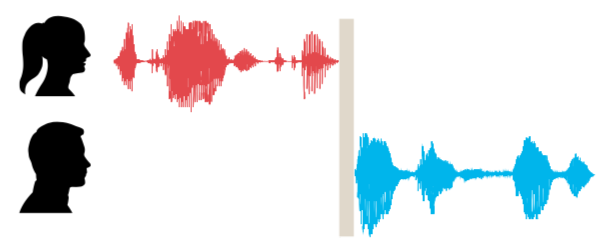
\includegraphics[width=\textwidth]{../aux/img/dummy_basic_concepts.png}
			\caption{Responses in conversation are fast\textsuperscript{[1]}}
		\end{figure}
	\end{columns}
	
	\vfill
	
	{\tiny\textsuperscript{[1]}\textsc{Levinson}, Stephen C.\ (2016): ``Turn-taking in human communication: Origins and implications for language processing.'' \textit{Trends in Cognitive Sciences} \textbf{20} (1): 6--14}
}
\frame{
	\frametitle{Turn-Taking -- Why do we care?}
	\begin{columns}
		\column{0.35\textwidth}
		\begin{itemize}
			\item present in related species
			\item human language universal
			\item present in early infancy
		\end{itemize}
		\column{0.65\textwidth}
		\begin{figure}
			% !TEX root = ../../beamer/ba_beamer_master.tex
% @author Marcel Ruland (2018)
\newcommand{\apewidth}{1.4cm}

\begin{tikzpicture}[
	every node/.append style={inner sep=0cm,align=center,text width=\apewidth,font=\tiny},
	node distance=0.1cm and 0.1cm,
]

%% top pics
\node							(lepilemur)		{\includegraphics[width=\apewidth]{../aux/img/species/lepilemur.jpg}};
\node[right=of lepilemur]		(callithrix)	{\includegraphics[width=\apewidth]{../aux/img/species/callithrix.jpg}};
\node[right=of callithrix]		(cebuella)		{\includegraphics[width=\apewidth]{../aux/img/species/cebuella.jpg}};
\node[right=of cebuella]		(callicebus)	{\includegraphics[width=\apewidth]{../aux/img/species/callicebus.jpg}};
\node[right=of callicebus]		(saimiri)		{\includegraphics[width=\apewidth]{../aux/img/species/saimiri.jpg}};
\node[right=of saimiri]			(cercopithecus)	{\includegraphics[width=\apewidth]{../aux/img/species/cercopithecus.png}};

%% bottom apes
\node[below=1.5cm of lepilemur]	(hylobates)		{\includegraphics[width=\apewidth]{../aux/img/species/hylobates.jpg}};
\node[right=of hylobates]		(orangutans)	{\includegraphics[width=\apewidth]{../aux/img/species/orangutans.jpg}};
\node[right=of orangutans]		(gorillas)		{\includegraphics[width=\apewidth]{../aux/img/species/gorillas.jpg}};
\node[right=of gorillas]		(chimpanzees)	{\includegraphics[width=\apewidth]{../aux/img/species/chimpanzees.png}};
\node[right=of chimpanzees]		(humans)		{\includegraphics[width=\apewidth]{../aux/img/species/humans.jpg}};
\node[right=of humans]			(diaemus)		{\includegraphics[width=\apewidth]{../aux/img/species/diaemus.jpg}};

%% braces
% prosimians
\draw[decorate,decoration={brace,amplitude=5pt}]
(lepilemur.north west) -- (lepilemur.north east)
node[midway,yshift=0.35cm]{\scriptsize{prosimians}};

% monkeys
\draw[decorate,decoration={brace,amplitude=5pt}]
(callithrix.north west) -- (cercopithecus.north east)
node[midway,yshift=0.35cm]{\scriptsize{monkeys}};

% apes
\draw[decorate,decoration={brace,amplitude=5pt}]
(humans.south east) -- (hylobates.south west)
node[midway,yshift=-0.35cm]{\scriptsize{apes}};

% bats
\draw[decorate,decoration={brace,amplitude=5pt}]
(diaemus.south east) -- (diaemus.south west)
node[midway,yshift=-0.35cm]{\scriptsize{bats}};

%% top labels
\node[below=of lepilemur]		{lepilemur edwardsi};
\node[below=of callithrix]		{callithrix jacchus};
\node[below=of cebuella]		{cebuella pygmaea};
\node[below=of callicebus]		{callicebus cupreus};
\node[below=of saimiri]			{saimiri};
\node[below=of cercopithecus]	{cercopithecus campbelli};

%% bottom labels
\node[above=of hylobates]		{hylobates syndactylus};
\node[above=of orangutans]		{orangutans};
\node[above=of gorillas]		{gorillas};
\node[above=of chimpanzees]		{chimpanzees};
\node[above=of humans]			{humans};
\node[above=of diaemus]			{diaemus youngi};
\end{tikzpicture}
			\caption{Turn-taking across species}
		\end{figure}
	\end{columns}
}


\section{Method}%%%%
\frame{
	\frametitle{Video Material}
	\begin{figure}
		\center
		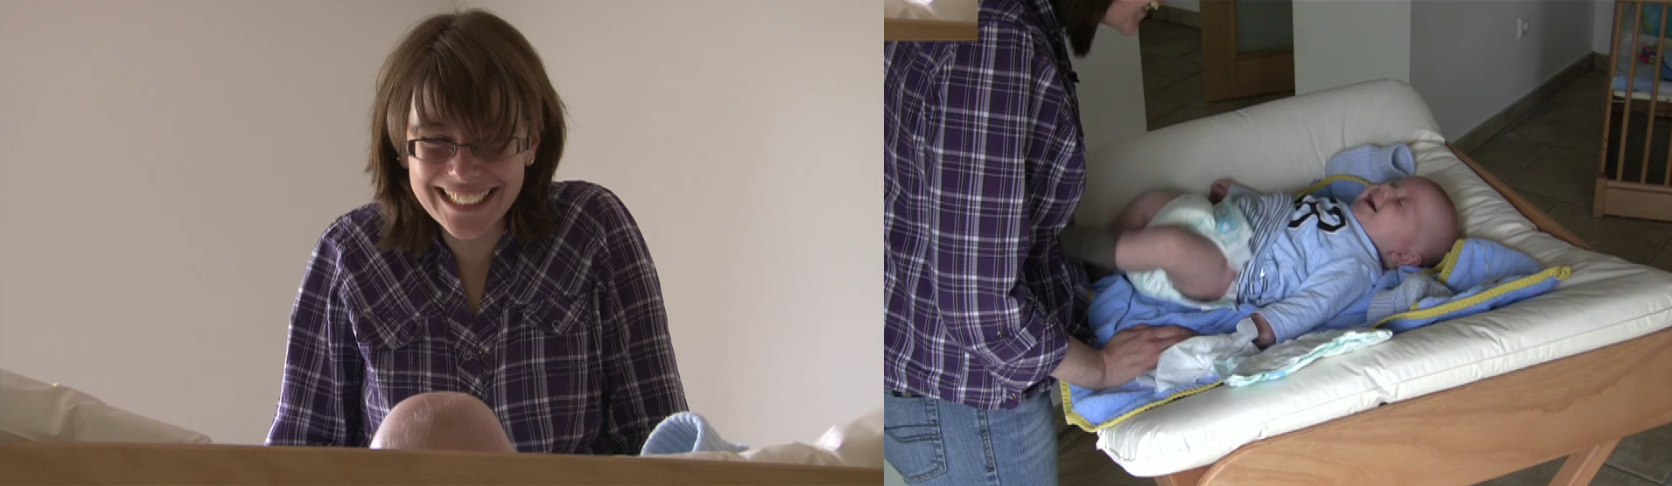
\includegraphics[width=\textwidth]{../aux/img/video_vp_08_compact.png}
		\caption{Example of recorded material}
	\end{figure}
}
\frame{
	\frametitle{Annotating the Videos}
	\only<+>{
		\begin{figure}
			\center
			\includegraphics[width=\textwidth]{../aux/img/elan.png}
			\caption{\textsc{elan} screenshot}
		\end{figure}
	}
	\only<+>{
		\begin{columns}
			\column{0.5\textwidth}
			\begin{itemize}
				\item intervals
				\item intervals from different modalities
				\item modalities from different sources
			\end{itemize}
			\column{0.5\textwidth}
			\begin{figure}
				\center
				\includegraphics[width=\textwidth]{../aux/img/elan_cropped.png}
				\caption{\textsc{elan} screenshot}
			\end{figure}
		\end{columns}
	}
}
\frame{
	\frametitle{What counts as a rule?}
	\begin{columns}
		\column{0.4\textwidth}
		\fpmlabel{A} \rightarrow \fpmlabel{B} represents one of two cases:\textsuperscript{[1]}
		\begin{enumerate}
			\item interval of \fpmlabel{A} starts before interval of \fpmlabel{B} \textbf{or}
			\item interval of \fpmlabel{A} and \fpmlabel{B} start at the same time
		\end{enumerate}
		\textbf{and} \fpmlabel{B} begins before \fpmlabel{A} ends
		\column{0.6\textwidth}
		\begin{figure}
			% !TEX root = ../../beamer/ba_beamer_master.tex
% @author Marcel Ruland (2018)
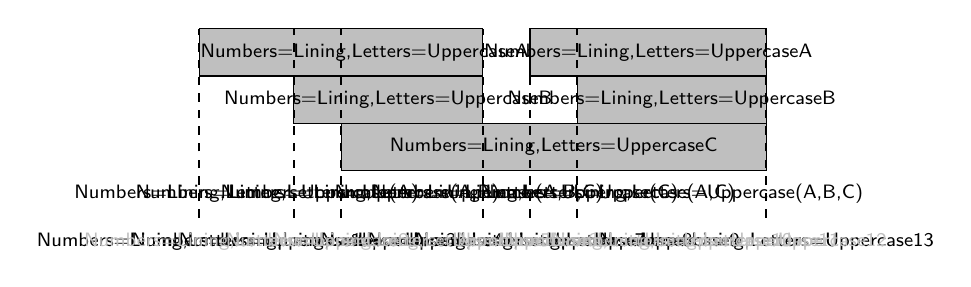
\begin{tikzpicture}[
	scale=0.6,
	every node/.append style={font=\scriptsize\sffamily\addfontfeature{Numbers=Lining,Letters=Uppercase}}]
	% boxes
	\draw [fill=lightgray] (0,4) rectangle (6,5);  % A1
	\node at (3.5,4.5) {A};
	
	\draw [fill=lightgray] (7,4) rectangle (12,5);  % A2
	\node at (9.5,4.5) {A};
	
	\draw [fill=lightgray] (2,3) rectangle (6,4);  % B1
	\node at (4,3.5) {B};
	
	\draw [fill=lightgray] (8,3) rectangle (12,4);  % B2
	\node at (10,3.5) {B};
	
	\draw [fill=lightgray] (3,2) rectangle (12,3);  % C
	\node at (7.5,2.5) {C};
	
	% item sets
	\node at (1,1.5) {(A)};
	\node at (2.5,1.5) {(A,B)};
	\node at (4.5,1.5) {(A,B,C)};
	\node at (6.5,1.5) {(C)};
	\node at (7.5,1.5) {(A,C)};
	\node at (10,1.5) {(A,B,C)};
	
	% time points
	\foreach \i in {1, 3, 4, 7, 8, 9, 13}
		\node at ({\i-1},0.5) {\i};
	\foreach \i in {2, 5, 6, 10, 11, 12}
		\node[lightgray] at ({\i-1},0.5) {\i};

	% time point lines
	\draw [dashed, thick] (0,1) -- (0,5);
	\draw [dashed, thick] (2,1) -- (2,5);
	\draw [dashed, thick] (3,1) -- (3,5);
	\draw [dashed, thick] (6,1) -- (6,5);
	\draw [dashed, thick] (7,1) -- (7,5);
	\draw [dashed, thick] (8,1) -- (8,5);
	\draw [dashed, thick] (12,1) -- (12,5);
\end{tikzpicture}
		\end{figure}
	\end{columns}
	
	\vfill
	
	{\tiny\textsuperscript{[1]}\textsc{Rohlfing}, Katharina; \textsc{Leonardi}, Giuseppe; \textsc{Hüllermeier}, Eyke; \textsc{Raczaszek-Leonardi}, Johanna; and \textsc{Nomikou}, Iris (under review): \\[-1em]
	``Multimodal turn-taking: Motivations, methodical challenges and first approaches.'' \textit{IEEE Transactions on Cognitive and Developmental Systems.}}
}
\frame{
	\frametitle{Metrics}
	\begin{columns}
		\column{0.4\textwidth}
		\begin{itemize}
			\item confidence \(conf(\mathcal{A} \rightarrow \mathcal{B}) = \frac{d(\mathcal{A}\cup\mathcal{B})}{d(\mathcal{A})}\)
			\item total number of occurrences
			\item duration (\textit{sec})
		\end{itemize}
		\column{0.6\textwidth}
		\begin{figure}
			% !TEX root = ../../beamer/ba_beamer_master.tex
% @author Marcel Ruland (2018)
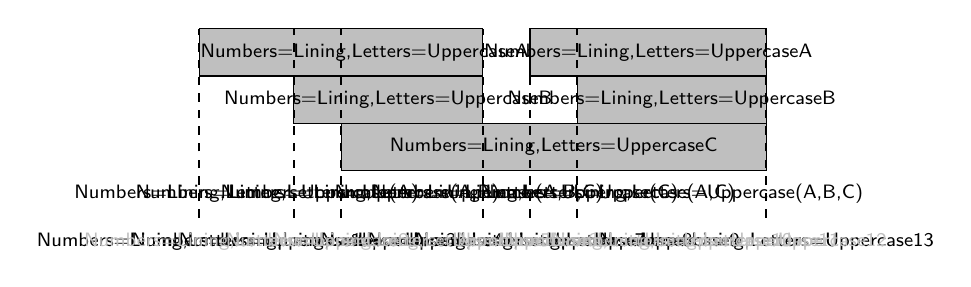
\begin{tikzpicture}[
	scale=0.6,
	every node/.append style={font=\scriptsize\sffamily\addfontfeature{Numbers=Lining,Letters=Uppercase}}]
	% boxes
	\draw [fill=lightgray] (0,4) rectangle (6,5);  % A1
	\node at (3.5,4.5) {A};
	
	\draw [fill=lightgray] (7,4) rectangle (12,5);  % A2
	\node at (9.5,4.5) {A};
	
	\draw [fill=lightgray] (2,3) rectangle (6,4);  % B1
	\node at (4,3.5) {B};
	
	\draw [fill=lightgray] (8,3) rectangle (12,4);  % B2
	\node at (10,3.5) {B};
	
	\draw [fill=lightgray] (3,2) rectangle (12,3);  % C
	\node at (7.5,2.5) {C};
	
	% item sets
	\node at (1,1.5) {(A)};
	\node at (2.5,1.5) {(A,B)};
	\node at (4.5,1.5) {(A,B,C)};
	\node at (6.5,1.5) {(C)};
	\node at (7.5,1.5) {(A,C)};
	\node at (10,1.5) {(A,B,C)};
	
	% time points
	\foreach \i in {1, 3, 4, 7, 8, 9, 13}
		\node at ({\i-1},0.5) {\i};
	\foreach \i in {2, 5, 6, 10, 11, 12}
		\node[lightgray] at ({\i-1},0.5) {\i};

	% time point lines
	\draw [dashed, thick] (0,1) -- (0,5);
	\draw [dashed, thick] (2,1) -- (2,5);
	\draw [dashed, thick] (3,1) -- (3,5);
	\draw [dashed, thick] (6,1) -- (6,5);
	\draw [dashed, thick] (7,1) -- (7,5);
	\draw [dashed, thick] (8,1) -- (8,5);
	\draw [dashed, thick] (12,1) -- (12,5);
\end{tikzpicture}
		\end{figure}
	\end{columns}
}


\section{Establishing Significance}%%%
\frame{
	\center
	{\Huge Why Significance?}
	\visible<2->{
		
		\vspace{0.2\textheight}
		
		\tikz\node[draw, rounded corners, inner sep=1em] {\LARGE qualitative \hspace{0.3\textwidth} quantitative};
	}
}
\frame{
	\frametitle{Significance -- How?}
	\begin{columns}
		\column{0.3\textwidth}
		\begin{enumerate}
			\item create 100 null distributions for every real sequence
			\item take 100 batches of 10: \\ 1 null distributions from each real distribution
			\item create distribution for every rule
			\item check real observation for significance against null observation distribution
		\end{enumerate}
		\column{0.7\textwidth}
		\only<+>{
			\begin{figure}
				% !TEX root = ../../beamer/ba_beamer_master.tex
% @author Marcel Ruland (2018)

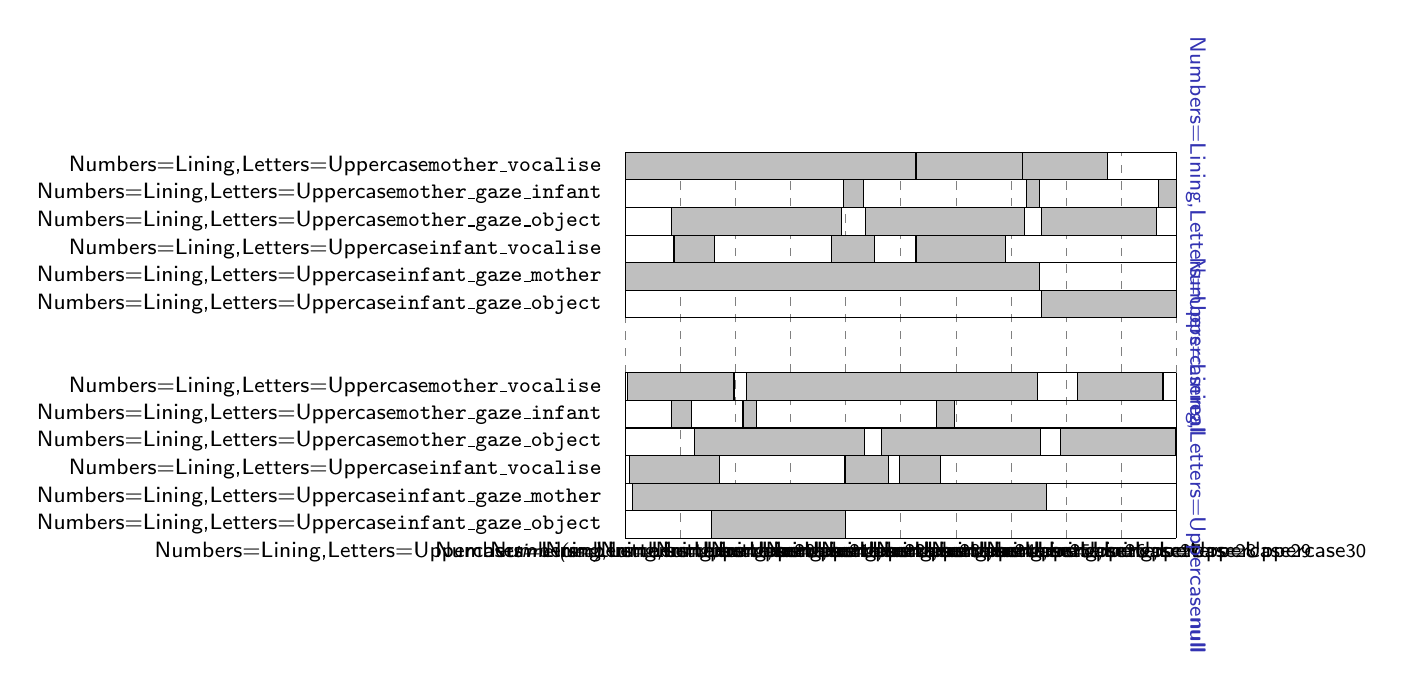
\begin{tikzpicture}[
	scale=0.7,  % a little smaller on beamer
	every node/.append style={font=\footnotesize\sffamily\addfontfeature{Numbers=Lining,Letters=Uppercase}}]
%	\draw [help lines] (0,0) grid (13,7);
	
	%% time line
	% annotations
	\node [anchor=east] at (2.75, -0.25) {\textit{\scriptsize{time (sec)}}};
	\foreach \i in {20, 21,..., 29, 30}
		\node at ({\i-17},-0.25) {\scriptsize{\i}};
	% small vertical help lines
	\draw [help lines, dashed] (3,3) -- (3,4);
	\draw [help lines, dashed] (13,3) -- (13,4);
	% long vertical help lines
	\foreach \i in {4, 5,..., 11, 12}
		\draw [help lines, dashed] (\i,0) -- (\i,7);
	
	%% grids
	% vertical lines
	\foreach \i in {3, 13}{
		\draw (\i,4) -- (\i,7);  % top
		\draw (\i,0) -- (\i,3);  % bottom
	}
	% horizontal lines
	\foreach \i in {0, 0.5,..., 2.5, 3, 4, 4.5,..., 6.5, 7}  % top and bottom
		\draw (3,\i) -- (13,\i);
	% annotations
	\node[color=beamerblue, rotate=-90, anchor=south] at (13,5.5) {\textbf{\textsc{real}}};
	\node[color=beamerblue, rotate=-90, anchor=south] at (13,1.5) {\textbf{\textsc{null}}};
		
	%% labels
	\foreach \i in {0.25, 4.25}{  % top and bottom
		\node[anchor=east] at (2.75,{\i+2.5}) {\code{mother\_vocalise}};
		\node[anchor=east] at (2.75,{\i+2}) {\code{mother\_gaze\_infant}};
		\node[anchor=east] at (2.75,{\i+1.5}) {\code{mother\_gaze\_object}};
		\node[anchor=east] at (2.75,{\i+1}) {\code{infant\_vocalise}};
		\node[anchor=east] at (2.75,{\i+0.5}) {\code{infant\_gaze\_mother}};
		\node[anchor=east] at (2.75,\i) {\code{infant\_gaze\_object}};
	}
	
	%% annotations
	% top
	\draw [fill=lightgray] (3,6.5) rectangle (8.279,7);
	\draw [fill=lightgray] (8.279,6.5) rectangle (10.206,7);
	\draw [fill=lightgray] (10.206,6.5) rectangle (11.76,7);

	\draw [fill=lightgray] (6.96,6) rectangle (7.32,6.5);
	\draw [fill=lightgray] (10.28,6) rectangle (10.52,6.5);
	\draw [fill=lightgray] (12.68,6) rectangle (13,6.5);
	
	\draw [fill=lightgray] (3.84,5.5) rectangle (6.92,6);
	\draw [fill=lightgray] (7.36,5.5) rectangle (10.24,6);
	\draw [fill=lightgray] (10.56,5.5) rectangle (12.64,6);
	
	\draw [fill=lightgray] (3.887,5) rectangle (4.624,5.5);
	\draw [fill=lightgray] (6.74,5) rectangle (7.53,5.5);
	\draw [fill=lightgray] (8.279,5) rectangle (9.909,5.5);
	
	\draw [fill=lightgray] (3,4.5) rectangle (10.52,5);

	\draw [fill=lightgray] (10.56,4) rectangle (13,4.5);
	% bottom
	\draw [fill=lightgray] (5.2,2.5) rectangle		({5.2+5.279},3);
	\draw [fill=lightgray] (3.05,2.5) rectangle		({3.05+1.927},3);
	\draw [fill=lightgray] (11.206,2.5) rectangle	({11.206+1.554},3);

	\draw [fill=lightgray] (3.84,2) rectangle		({3.84+0.36},2.5);
	\draw [fill=lightgray] (5.14,2) rectangle		({5.14+0.24},2.5);
	\draw [fill=lightgray] (8.65,2) rectangle		({8.65+0.32},2.5);
	
	\draw [fill=lightgray] (4.26,1.5) rectangle		({4.26+3.08},2);
	\draw [fill=lightgray] (7.66,1.5) rectangle		({7.66+2.88},2);
	\draw [fill=lightgray] (10.9,1.5) rectangle		({10.9+2.08},2);
	
	\draw [fill=lightgray] (7.987,1) rectangle		({7.987+0.737},1.5);
	\draw [fill=lightgray] (6.99,1) rectangle		({6.99+0.79},1.5);
	\draw [fill=lightgray] (3.079,1) rectangle		({3.079+1.63},1.5);
	
	\draw [fill=lightgray] (3.13,0.5) rectangle		({3.13+7.52},1);

	\draw [fill=lightgray] (4.56,0) rectangle		({4.56+2.44},0.5);
\end{tikzpicture}
			\end{figure}
		}
		\only<+>{
			\begin{figure}
				% !TEX root = ../../beamer/ba_beamer_master.tex
% @author Marcel Ruland (2018)

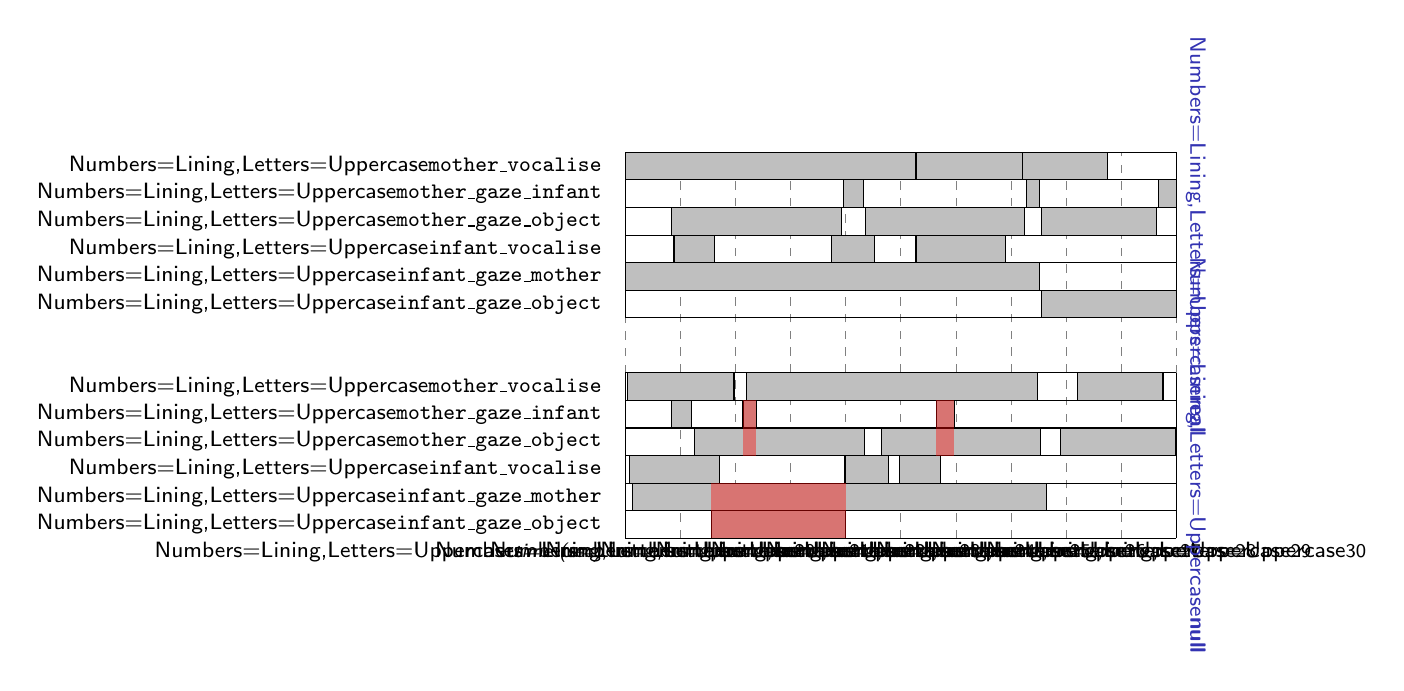
\begin{tikzpicture}[
	scale=0.7,  % a little smaller on beamer
	every node/.append style={font=\footnotesize\sffamily\addfontfeature{Numbers=Lining,Letters=Uppercase}}]
%	\draw [help lines] (0,0) grid (13,7);
	
	%% time line
	% annotations
	\node [anchor=east] at (2.75, -0.25) {\textit{\scriptsize{time (sec)}}};
	\foreach \i in {20, 21,..., 29, 30}
		\node at ({\i-17},-0.25) {\scriptsize{\i}};
	% small vertical help lines
	\draw [help lines, dashed] (3,3) -- (3,4);
	\draw [help lines, dashed] (13,3) -- (13,4);
	% long vertical help lines
	\foreach \i in {4, 5,..., 11, 12}
		\draw [help lines, dashed] (\i,0) -- (\i,7);
	
	%% grids
	% vertical lines
	\foreach \i in {3, 13}{
		\draw (\i,4) -- (\i,7);  % top
		\draw (\i,0) -- (\i,3);  % bottom
	}
	% horizontal lines
	\foreach \i in {0, 0.5,..., 2.5, 3, 4, 4.5,..., 6.5, 7}  % top and bottom
		\draw (3,\i) -- (13,\i);
	% annotations
	\node[color=beamerblue, rotate=-90, anchor=south] at (13,5.5) {\textbf{\textsc{real}}};
	\node[color=beamerblue, rotate=-90, anchor=south] at (13,1.5) {\textbf{\textsc{null}}};
		
	%% labels
	\foreach \i in {0.25, 4.25}{  % top and bottom
		\node[anchor=east] at (2.75,{\i+2.5}) {\code{mother\_vocalise}};
		\node[anchor=east] at (2.75,{\i+2}) {\code{mother\_gaze\_infant}};
		\node[anchor=east] at (2.75,{\i+1.5}) {\code{mother\_gaze\_object}};
		\node[anchor=east] at (2.75,{\i+1}) {\code{infant\_vocalise}};
		\node[anchor=east] at (2.75,{\i+0.5}) {\code{infant\_gaze\_mother}};
		\node[anchor=east] at (2.75,\i) {\code{infant\_gaze\_object}};
	}
	
	%% annotations
	% top
	\draw [fill=lightgray] (3,6.5) rectangle (8.279,7);
	\draw [fill=lightgray] (8.279,6.5) rectangle (10.206,7);
	\draw [fill=lightgray] (10.206,6.5) rectangle (11.76,7);

	\draw [fill=lightgray] (6.96,6) rectangle (7.32,6.5);
	\draw [fill=lightgray] (10.28,6) rectangle (10.52,6.5);
	\draw [fill=lightgray] (12.68,6) rectangle (13,6.5);
	
	\draw [fill=lightgray] (3.84,5.5) rectangle (6.92,6);
	\draw [fill=lightgray] (7.36,5.5) rectangle (10.24,6);
	\draw [fill=lightgray] (10.56,5.5) rectangle (12.64,6);
	
	\draw [fill=lightgray] (3.887,5) rectangle (4.624,5.5);
	\draw [fill=lightgray] (6.74,5) rectangle (7.53,5.5);
	\draw [fill=lightgray] (8.279,5) rectangle (9.909,5.5);
	
	\draw [fill=lightgray] (3,4.5) rectangle (10.52,5);

	\draw [fill=lightgray] (10.56,4) rectangle (13,4.5);
	% bottom
	\draw [fill=lightgray] (5.2,2.5) rectangle		({5.2+5.279},3);
	\draw [fill=lightgray] (3.05,2.5) rectangle		({3.05+1.927},3);
	\draw [fill=lightgray] (11.206,2.5) rectangle	({11.206+1.554},3);

	\draw [fill=lightgray] (3.84,2) rectangle		({3.84+0.36},2.5);
	\draw [fill=lightgray] (5.14,2) rectangle		({5.14+0.24},2.5);
	\draw [fill=lightgray] (8.65,2) rectangle		({8.65+0.32},2.5);
	
	\draw [fill=lightgray] (4.26,1.5) rectangle		({4.26+3.08},2);
	\draw [fill=lightgray] (7.66,1.5) rectangle		({7.66+2.88},2);
	\draw [fill=lightgray] (10.9,1.5) rectangle		({10.9+2.08},2);
	
	\draw [fill=lightgray] (7.987,1) rectangle		({7.987+0.737},1.5);
	\draw [fill=lightgray] (6.99,1) rectangle		({6.99+0.79},1.5);
	\draw [fill=lightgray] (3.079,1) rectangle		({3.079+1.63},1.5);
	
	\draw [fill=lightgray] (3.13,0.5) rectangle		({3.13+7.52},1);

	\draw [fill=lightgray] (4.56,0) rectangle		({4.56+2.44},0.5);
	% red
	\fill [alert, opacity=0.4] (8.65,1.5) rectangle ({8.65+0.32},2.5);
	\fill [alert, opacity=0.4] (5.14,1.5) rectangle ({5.14+0.24},2.5);
	\fill [alert, opacity=0.4] (4.56,0) rectangle ({4.56+2.44},1);
\end{tikzpicture}
			\end{figure}
		}
		\only<+>{
			\begin{figure}
				% !TEX root = ../../beamer/ba_beamer_master.tex
% @author Marcel Ruland (2018)

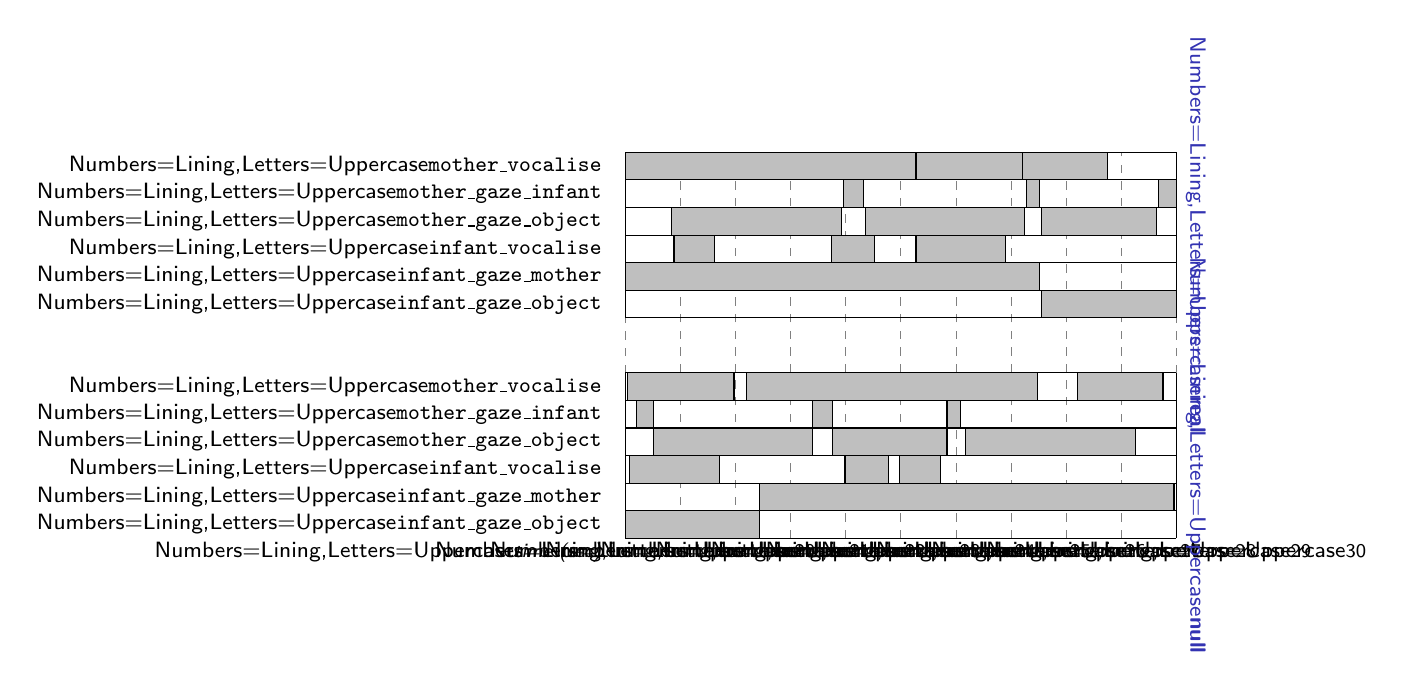
\begin{tikzpicture}[
	scale=0.7,  % a little smaller on beamer
	every node/.append style={font=\footnotesize\sffamily\addfontfeature{Numbers=Lining,Letters=Uppercase}}]
%	\draw [help lines] (0,0) grid (13,7);
	
	%% time line
	% annotations
	\node [anchor=east] at (2.75, -0.25) {\textit{\scriptsize{time (sec)}}};
	\foreach \i in {20, 21,..., 29, 30}
		\node at ({\i-17},-0.25) {\scriptsize{\i}};
	% small vertical help lines
	\draw [help lines, dashed] (3,3) -- (3,4);
	\draw [help lines, dashed] (13,3) -- (13,4);
	% long vertical help lines
	\foreach \i in {4, 5,..., 11, 12}
		\draw [help lines, dashed] (\i,0) -- (\i,7);
	
	%% grids
	% vertical lines
	\foreach \i in {3, 13}{
		\draw (\i,4) -- (\i,7);  % top
		\draw (\i,0) -- (\i,3);  % bottom
	}
	% horizontal lines
	\foreach \i in {0, 0.5,..., 2.5, 3, 4, 4.5,..., 6.5, 7}  % top and bottom
		\draw (3,\i) -- (13,\i);
	% annotations
	\node[color=beamerblue, rotate=-90, anchor=south] at (13,5.5) {\textbf{\textsc{real}}};
	\node[color=beamerblue, rotate=-90, anchor=south] at (13,1.5) {\textbf{\textsc{null}}};
		
	%% labels
	\foreach \i in {0.25, 4.25}{  % top and bottom
		\node[anchor=east] at (2.75,{\i+2.5}) {\code{mother\_vocalise}};
		\node[anchor=east] at (2.75,{\i+2}) {\code{mother\_gaze\_infant}};
		\node[anchor=east] at (2.75,{\i+1.5}) {\code{mother\_gaze\_object}};
		\node[anchor=east] at (2.75,{\i+1}) {\code{infant\_vocalise}};
		\node[anchor=east] at (2.75,{\i+0.5}) {\code{infant\_gaze\_mother}};
		\node[anchor=east] at (2.75,\i) {\code{infant\_gaze\_object}};
	}
	
	%% annotations
	% top
	\draw [fill=lightgray] (3,6.5) rectangle (8.279,7);
	\draw [fill=lightgray] (8.279,6.5) rectangle (10.206,7);
	\draw [fill=lightgray] (10.206,6.5) rectangle (11.76,7);

	\draw [fill=lightgray] (6.96,6) rectangle (7.32,6.5);
	\draw [fill=lightgray] (10.28,6) rectangle (10.52,6.5);
	\draw [fill=lightgray] (12.68,6) rectangle (13,6.5);
	
	\draw [fill=lightgray] (3.84,5.5) rectangle (6.92,6);
	\draw [fill=lightgray] (7.36,5.5) rectangle (10.24,6);
	\draw [fill=lightgray] (10.56,5.5) rectangle (12.64,6);
	
	\draw [fill=lightgray] (3.887,5) rectangle (4.624,5.5);
	\draw [fill=lightgray] (6.74,5) rectangle (7.53,5.5);
	\draw [fill=lightgray] (8.279,5) rectangle (9.909,5.5);
	
	\draw [fill=lightgray] (3,4.5) rectangle (10.52,5);

	\draw [fill=lightgray] (10.56,4) rectangle (13,4.5);
	% bottom
	\draw [fill=lightgray] (5.2,2.5) rectangle		({5.2+5.279},3);
	\draw [fill=lightgray] (3.05,2.5) rectangle		({3.05+1.927},3);
	\draw [fill=lightgray] (11.206,2.5) rectangle	({11.206+1.554},3);

	\draw [fill=lightgray] (6.4,2) rectangle		({6.4+0.36},2.5);
	\draw [fill=lightgray] (8.84,2) rectangle		({8.84+0.24},2.5);
	\draw [fill=lightgray] (3.2,2) rectangle		({3.2+0.32},2.5);
	
	\draw [fill=lightgray] (9.18,1.5) rectangle		({9.18+3.08},2);
	\draw [fill=lightgray] (3.52,1.5) rectangle		({3.52+2.88},2);
	\draw [fill=lightgray] (6.76,1.5) rectangle		({6.76+2.08},2);
	
	\draw [fill=lightgray] (7.987,1) rectangle		({7.987+0.737},1.5);
	\draw [fill=lightgray] (6.99,1) rectangle		({6.99+0.79},1.5);
	\draw [fill=lightgray] (3.079,1) rectangle		({3.079+1.63},1.5);
	
	\draw [fill=lightgray] (5.44,0.5) rectangle		({5.44+7.52},1);

	\draw [fill=lightgray] (3,0) rectangle			({3+2.44},0.5);
\end{tikzpicture}
			\end{figure}
		}
	\end{columns}
}

\section{Interpretation}
\frame{
	\frametitle{Interpretation}
	\begin{columns}
		\column{0.5\textwidth}
		{\color{beamerblue} Things to Keep in Mind}
		\begin{itemize}
			\item evaluate in context
			\item mothers (almost) always talk \\ ~
			\item[]~
		\end{itemize}
		\column{0.5\textwidth}
		{\color{beamerblue} Things to Look for}
		\begin{itemize}
			\item confirming existing research
			\item new ``interesting'' rules (whatever that means)
			\item generate new hypotheses
		\end{itemize}
	\end{columns}
}
\frame{
	\begin{columns}
		\column{0.65\textwidth}
		\center
		{\Huge Thank you.}
		\column{0.35\textwidth}
		{\color{beamerblue} Picture Credits}
		\begin{tabularx}{\textwidth}{>{\bfseries\tiny}r>{\tiny}X}
			lepilemur edwardsi & \copyright\ Frank Vassen \\
			callithrix jacchus & \copyright\ Raimond Spekking \\
			cebuella pygmaea & \copyright\ Don Faulkner \\
			callicebus cupreus & \copyright\ Udo Schröter \\
			saimiri & \copyright\ Ernst Vikne \\
			hylobates syndactylus & \copyright\ Su Neko\\
			orangutan & \copyright\ Trisha Shears \\
			chimpanzee & \copyright\ Frans de Waal \\
			human & \copyright\ Jelly Helm \\
		\end{tabularx}
	\end{columns}
}
\end{document}
